\documentclass{article}
\usepackage{tikz}
\usetikzlibrary{arrows.meta, positioning, calc, automata, shapes.geometric}

\begin{document}
	
	\section{Schematische Darstellung eines Variational Autoencoders (VAE)}
	
	\begin{figure}[h]
		\centering
		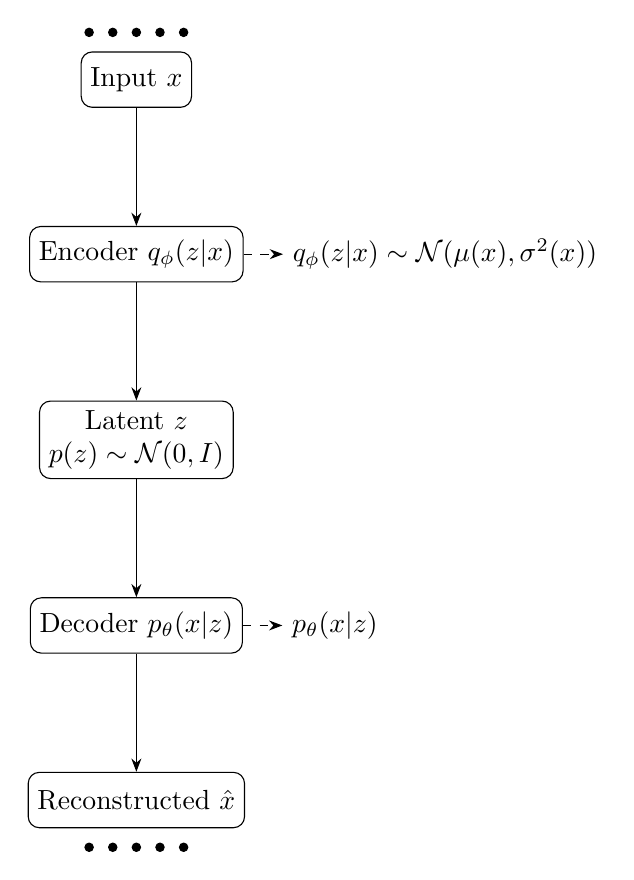
\begin{tikzpicture}[
			node distance=1.5cm and 2cm,
			every node/.style={align=center},
			box/.style={rectangle, draw, rounded corners, minimum height=2em, minimum width=3em},
			dot/.style={circle, draw, fill=black, inner sep=0pt, minimum size=3pt},
			>=Stealth
			]
			% Nodes
			\node[box] (input) {Input $x$};
			\node[box, below=of input] (encoder) {Encoder $q_\phi(z|x)$};
			\node[box, below=of encoder] (latent) {Latent $z$\\$p(z) \sim \mathcal{N}(0, I)$};
			\node[box, below=of latent] (decoder) {Decoder $p_\theta(x|z)$};
			\node[box, below=of decoder] (reconstructed) {Reconstructed $\hat{x}$};
			
			% Arrows
			\draw[->] (input) -- (encoder);
			\draw[->] (encoder) -- (latent);
			\draw[->] (latent) -- (decoder);
			\draw[->] (decoder) -- (reconstructed);
			
			% Descriptions
			\node[right=0.5cm of encoder] (q) {$q_\phi(z|x) \sim \mathcal{N}(\mu(x), \sigma^2(x))$};
			\node[right=0.5cm of decoder] (p) {$p_\theta(x|z)$};
			
			\draw[->, dashed] (encoder) -- (q);
			\draw[->, dashed] (decoder) -- (p);
			
			% Data points
			\foreach \i in {-0.6, -0.3, 0, 0.3, 0.6} {
				\node[dot] at ($(input) + (\i, 0.6)$) {};
				\node[dot] at ($(reconstructed) + (\i, -0.6)$) {};
			}
		\end{tikzpicture}
		\caption{Schematische Darstellung eines Variational Autoencoders (VAE) mit Datenpunkten}
		\label{fig:vae}
	\end{figure}
	
	
\begin{figure}[h]
	\centering
	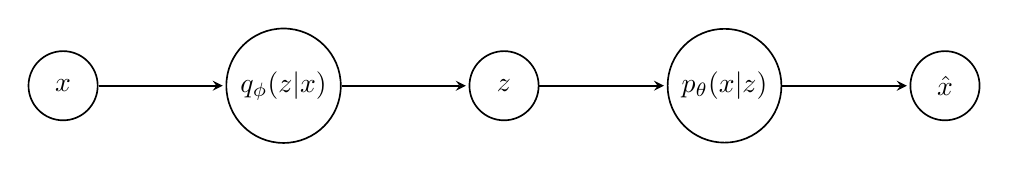
\begin{tikzpicture}[->,>=stealth,shorten >=1pt,auto,node distance=2.8cm, semithick]
		\tikzstyle{every state}=[fill=none,draw=black,text=black]
		
		\node[state] (A)                    {$x$};
		\node[state] (B) [right of=A]       {$q_\phi(z|x)$};
		\node[state] (C) [right of=B]       {$z$};
		\node[state] (D) [right of=C]       {$p_\theta(x|z)$};
		\node[state] (E) [right of=D]       {$\hat{x}$};
		
		\path (A) edge node {} (B)
		(B) edge node {} (C)
		(C) edge node {} (D)
		(D) edge node {} (E);
	\end{tikzpicture}
	\caption{Schematische Darstellung eines Variational Autoencoders (VAE)}
	\label{fig:vae}
\end{figure}

\begin{figure}[h]
	\centering
	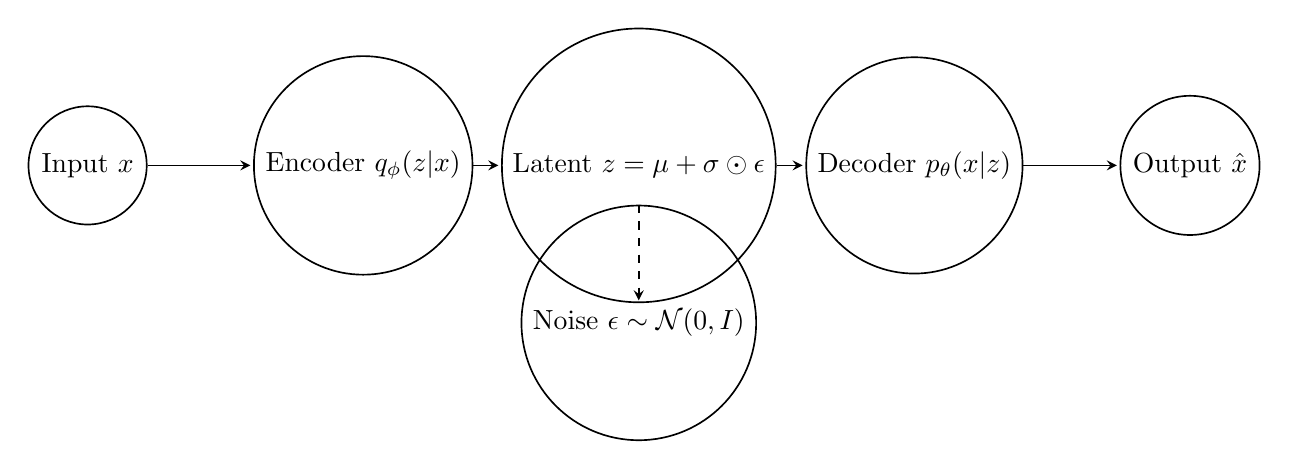
\begin{tikzpicture}[->,>=stealth,shorten >=1pt,auto,node distance=3.5cm, semithick]
		\tikzstyle{every state}=[fill=none,draw=black,text=black]
		
		\node[state] (A)                    {Input $x$};
		\node[state] (B) [right of=A]       {Encoder $q_\phi(z|x)$};
		\node[state] (C) [right of=B]       {Latent $z = \mu + \sigma \odot \epsilon$};
		\node[state] (D) [right of=C]       {Decoder $p_\theta(x|z)$};
		\node[state] (E) [right of=D]       {Output $\hat{x}$};
		\node[state] (F) [below of=C, node distance=2cm] {Noise $\epsilon \sim \mathcal{N}(0, I)$};
		
		\path (A) edge node {} (B)
		(B) edge node {} (C)
		(C) edge node {} (D)
		(D) edge node {} (E);
		\path[dashed] (F) edge node {} (C);
	\end{tikzpicture}
	\caption{Schematische Darstellung des Reparameterization-Tricks in einem Variational Autoencoder (VAE)}
	\label{fig:reparam_trick}
\end{figure}


\begin{figure}[h]
	\centering
	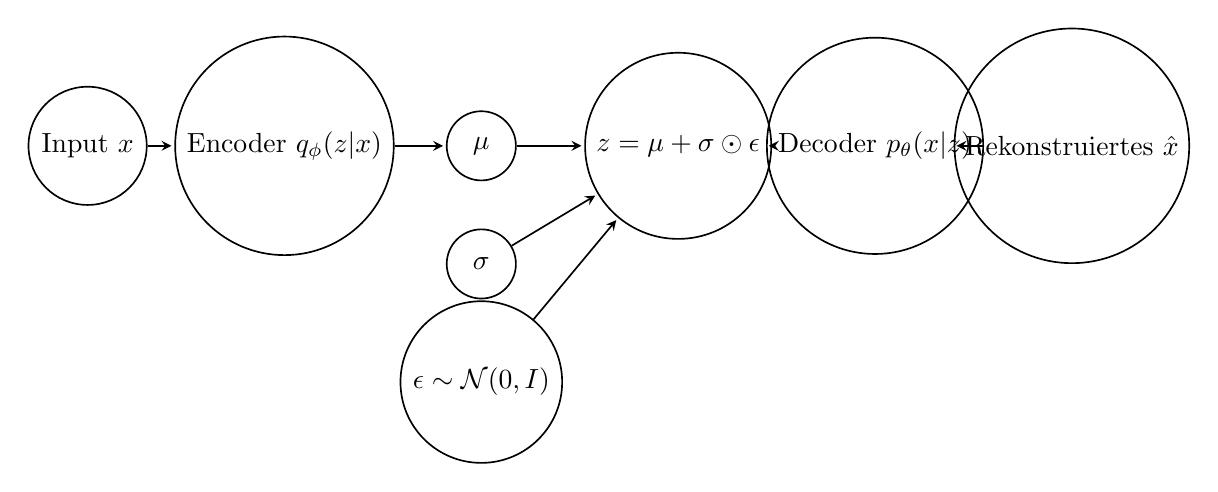
\begin{tikzpicture}[->,>=stealth,shorten >=1pt,auto,node distance=2.5cm, semithick]
		\tikzstyle{every state}=[fill=none,draw=black,text=black]
		
		\node[state] (A)                    {Input $x$};
		\node[state] (B) [right of=A]       {Encoder $q_\phi(z|x)$};
		\node[state] (C) [right of=B]       { $\mu$};
		\node[state] (D) [below of=C, node distance=1.5cm] { $\sigma$};
		\node[state] (E) [below of=D, node distance=1.5cm] { $\epsilon \sim \mathcal{N}(0, I)$};
		\node[state] (F) [right of=C, node distance=2.5cm] { $z = \mu + \sigma \odot \epsilon$};
		\node[state] (G) [right of=F, node distance=2.5cm] {Decoder $p_\theta(x|z)$};
		\node[state] (H) [right of=G, node distance=2.5cm] {Rekonstruiertes $\hat{x}$};
		
		\path (A) edge node {} (B)
		(B) edge node {} (C)
		(C) edge node {} (F)
		(D) edge node {} (F)
		(E) edge node {} (F)
		(F) edge node {} (G)
		(G) edge node {} (H);
	\end{tikzpicture}
	\caption{Schematische Darstellung des Reparameterization-Tricks in einem Variational Autoencoder (VAE)}
	\label{fig:reparam_trick}
\end{figure}

\begin{figure}[h]
	\centering
	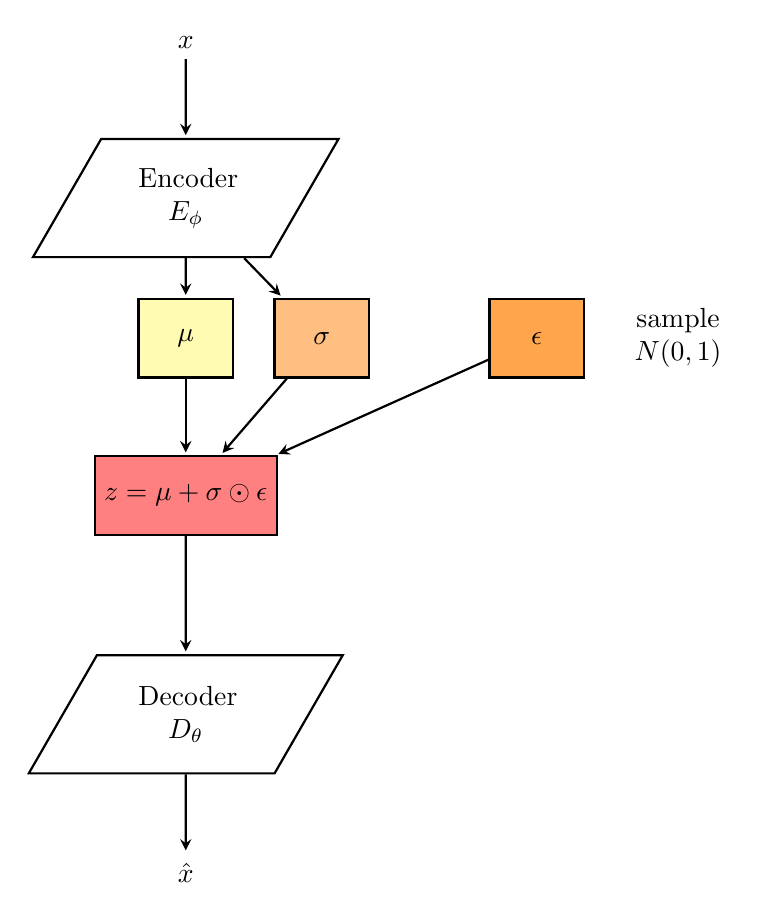
\begin{tikzpicture}[->,>=stealth,shorten >=1pt,auto,node distance=1.5cm, thick]
		
		% Input x
		\node (x) {$x$};
		
		% Encoder block
		\node[draw, trapezium, trapezium left angle=60, trapezium right angle=120, minimum height=1.5cm, text width=1.2cm, align=center, below=1cm of x] (encoder) {Encoder\\$E_\phi$};
		
		% Mean and standard deviation
		\node[draw, rectangle, fill=yellow!30, below=0.5cm of encoder, minimum height=1cm, minimum width=1.2cm] (mu) {$\mu$};
		\node[draw, rectangle, fill=orange!50, below=0.5cm of encoder, right=0.5 of mu, minimum height=1cm, minimum width=1.2cm] (sigma) {$\sigma$};
		
		% Latent variable z
		\node[draw, rectangle, fill=red!50, below=2.5cm of encoder, minimum height=1cm, minimum width=1.2cm] (z) { $z = \mu + \sigma \odot \epsilon$};
		
		% Noise epsilon
		\node[draw, rectangle, fill=orange!70, right=1.5cm of sigma, minimum height=1cm, minimum width=1.2cm] (epsilon) {$\epsilon$};
		\node[align=center, right=0.5cm of epsilon] {sample\\$N(0,1)$};
		
		% Decoder block
		\node[draw, trapezium, trapezium left angle=60, trapezium right angle=120, minimum height=1.5cm, text width=1.2cm, align=center, below=1.5cm of z] (decoder) {Decoder\\$D_\theta$};
		
		% Output x_hat
		\node[below=1cm of decoder] (x_hat) {$\hat{x}$};
				
		% Connections
		\draw[->] (x) -- (encoder);
		\draw[->] (encoder) -- (mu);
		\draw[->] (encoder) -- (sigma);
		\draw[->] (mu) -- (z);
		\draw[->] (sigma) -- (z);
		\draw[->] (epsilon) -- (z);
		\draw[->] (z) -- (decoder);
		\draw[->] (decoder) -- (x_hat);
		

		
	\end{tikzpicture}
	\caption{Schematische Darstellung des Reparameterization-Tricks in einem Variational Autoencoder (VAE)}
	\label{fig:reparam_trick}
\end{figure}
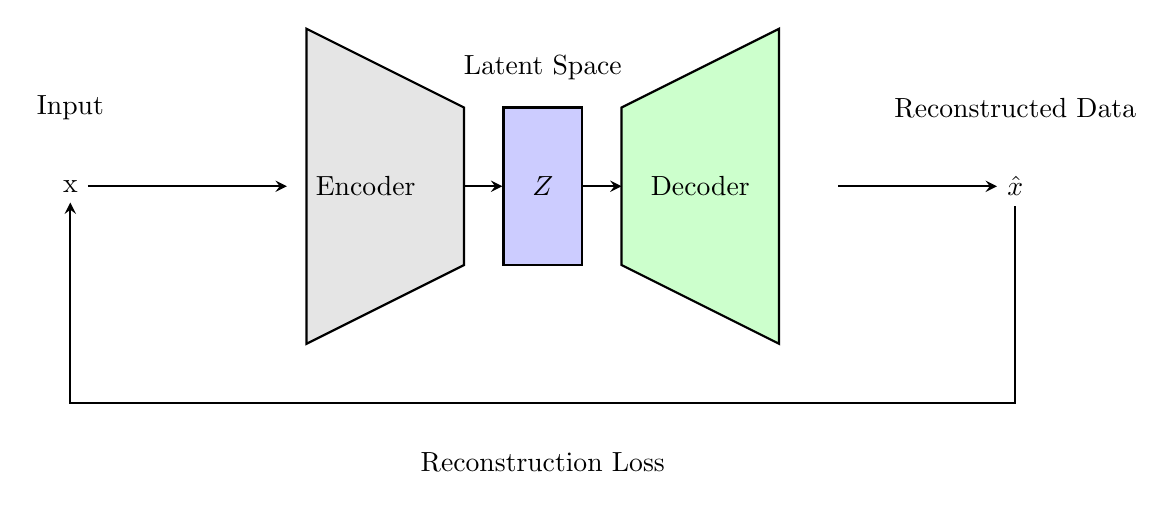
\begin{tikzpicture}[auto, thick, node distance=2cm, >=stealth]
	
	% Define styles
	\tikzstyle{latent} = [rectangle, draw, fill=blue!20, text centered, minimum width=1cm, minimum height=2cm]
	\tikzstyle{input} = [rectangle, text centered]
	\tikzstyle{output} = [rectangle, text centered]
	
	% Nodes
	\node[input, name=input] (input) {x};
	\node[latent, right of=input, node distance=6cm, minimum width=1cm, minimum height=2cm] (z) {$Z$};
	\node[output, right of=z, node distance=6cm] (output) {$\hat{x}$};
	
	% Custom trapezoids for encoder and decoder
	\draw[fill=gray!20] (3,2) -- (3,-2) -- (5,-1) -- (5,1) -- cycle;
	\node at (3.75, 0) {Encoder};
	
	\draw[fill=green!20] (7,1) -- (7,-1) -- (9,-2) -- (9,2) -- cycle;
	\node at (8, 0) {Decoder};
	
	% Arrows
	\draw[->] (input.east) -- (2.75,0);
	\draw[->] (5,0) -- (z.west);
	\draw[->] (z.east) -- (7,0);
	\draw[->] (9.75,0) -- (output.west);
	
	% Labels
	\node[above of=input, node distance=1cm] {Input};
	\node[above of=z, node distance=1.5cm] {Latent Space};
	\node[above of=output, node distance=1cm] {Reconstructed Data};
	
	% Additional Text
	\draw[->, thick] (output.south) |- ++(0, -2.5cm) -| (input.south);
	\node[below of=z, node distance=3.5cm, text width=6cm, align=center] {Reconstruction Loss};
	
\end{tikzpicture}

\begin{tikzpicture}[auto, thick, node distance=2cm, >=stealth]
	
	% Define block styles
	\tikzstyle{block} = [trapezium, trapezium left angle=70, trapezium right angle=110, minimum height=3cm, draw, fill=gray!20, text centered]
	\tikzstyle{block2} = [trapezium, trapezium left angle=110, trapezium right angle=70, minimum height=3cm, draw, fill=green!20, text centered]
	\tikzstyle{square} = [rectangle, draw, fill=red!20, minimum size=1.5cm, text centered]
	\tikzstyle{latent} = [rectangle, draw, fill=blue!20, minimum size=1.5cm, text centered]
	
	% Nodes	
	\draw[fill=gray!20] (1,2) -- (1,-2) -- (3,-1) -- (3,1) -- cycle;
	\node[right of=input, node distance=2cm] (encoder) {$q_{\phi}(z \mid x)$};
	\node[rectangle, draw, fill=yellow!20, minimum height=3cm, minimum width=1cm, text centered] (input) {$\mathbf{x}$};
	\node[square, right of=encoder, node distance=2.5cm] (mu) {$\mu_{z|x}$};
	\node[square, below of=mu, node distance=2cm] (sigma) {$\Sigma_{z|x}$};
	\node[latent, right of=mu, node distance=2cm] (z) {$\mathbf{Z}$};
	\draw[fill=green!20] (8,1) -- (8,-1) -- (10,-2) -- (10,2) -- cycle;
	\node[right of=z, node distance=2.5cm] (decoder) { $p_{\theta}(x \mid z)$};	
	\node[rectangle, draw, fill=yellow!20, minimum height=3cm, minimum width=1cm, text centered, right of=decoder, node distance=3cm] (output) {$\hat{\mathbf{x}}$};
	


	% Arrows
	\draw[->] (input) -- (1,0);
	\draw[->] (3,0) -- (mu);
	\draw[->] (3,0) -- (sigma);
	\draw[->] (mu) -- (z);
	\draw[->] (sigma) -- (z);
	\draw[->] (z) -- (8,0);
	\draw[->] (10,0) -- (output);
	
	% Labels
	\node[above of=input, node distance=1.75cm] {Input Data};
	\node[above of=encoder, node distance=0.8cm] {Encoder};
	\node[above of=z, node distance=1cm] {Latent Space};
	\node[above of=decoder, node distance=0.8cm] {Decoder};
	\node[above of=output, node distance=1.75cm] {Reconstructed Image};
	
	\node[below of=sigma, node distance=1.2cm] {Standard Deviation};
	
	% Additional Text
	\draw[->, thick] (input.south) |- ++(0, -2.5cm) -| (output.south);
	\node[below of=encoder, node distance=4.5cm, text width=6cm, align=center] {Reconstruction Loss + KL Divergence};
	
\end{tikzpicture}
\end{document}